%%==================================================
%% chapter01.tex for BIT Master Thesis
%% modified by pinren lu
%% version: 0.1
%% last update: Dec 25th, 2016
%%==================================================
% 相关工作

% 1. 文本生成技术
% 2. 大语言模型生成技术
% 3. 文本分类技术
% 4. 大语言模型文本探测技术
% 5. 本章小结

\chapter{相关工作}
\label{chap:related works}

\section{文本生成技术}
\label{sec:rw-lm}

在当前的自然语言处理领域,主流的大语言模型普遍采用了 Transformer 框架 \cite{transformer}。这一架构自 2017 年提出以来,因其卓越的并行处理能力和长距离依赖建模能力而迅速成为研究的热点。Transformer 通过自注意力机制有效捕捉输入序列中各个部分之间的关系,使得模型能够在处理大规模文本数据时,显著提高了训练效率和表达能力。诸如 BERT、GPT 系列等知名模型,均基于这一框架,展现出了在多种语言任务上优异的性能。因此,深入探讨 Transformer 的结构与原理,不仅有助于理解当前大语言模型的成功之处,也为未来的研究提供了重要的理论基础。

Transformer 是 Google 于 2017 年提出的一种基于自注意力机制的用于处理 Seq2Seq 任务的神经网络模型,被广泛用于各种 NLP 任务中。Transformer 利用自注意力机制来处理输入序列中的关联性,能够有效地捕捉长距离依赖关系,无需依赖于循环神经网络或卷积神经网络。同时,Transformer 可以并行地处理输入序列中的不同位置,因此在训练和推理时,特别是在处理长序列时具有更高的效率。

\begin{figure}[htbp]
	\centering
	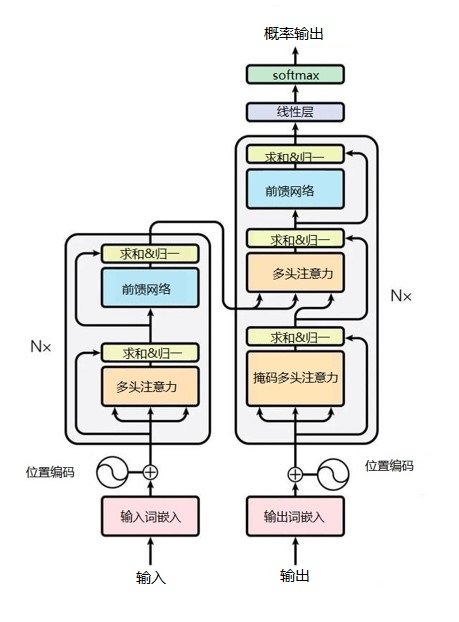
\includegraphics[scale = 0.8]{figures/Transformer2}
	\caption{Transformer 模型结构}
	\label{fig:Transformer2}
\end{figure}

\subsection{编码器-解码器结构}

(1) 编码器

编码器有 $N=6$ 个完全一样的 TransformerEncoderLayer 层。在每一个 TransformerEncoderLayer 层中,可以将每一层分成两个子层。第一个子层是多头的自注意力机制,第二个子层仅仅只是朴素的位置全连接前馈网络。这两个子层中,每一个子层后面都要接一个残差连接网络,这之后再把经过残差连接层的变量进行归一化。简言之,每一个子层输出出来的向量实际上是 $\text{LayerNormal}(x + \text{Sublayer}(x))$,上式中 $\text{Sublayer}(x)$ 表示的是每一个子层自己实现的功能。为了使得残差连接的维度数相等以及方便残差连接计算等一系列原因,上述模型中的所有子层以及嵌入层的输出向量的维度数量都为 $d_{\text{model}} = 512$。

(2) 解码器

解码器也有 $N = 6$ 个完全一样的 TransformerDecoderLayer 层。在每一个 TransformerDecoderLayer 层中,包含了三个子层。其中两个子层与编码器层中的子层大体相似,而第三个子层,这个子层输入编码器堆栈的输出且输入解码器层的上一个多头注意力子层的输出,并在该子层内执行多头注意力操作。与编码器层中的子层的结构类似,把残差连接网络接到每一个解码器层的子层后面,这之后再把经过残差连接层的变量进行层归一化。本课题也修改了解码器结构中的自注意力子层,加入了位置掩码,这样可以防止出现从前面的某个位置获得后面某个位置的信息。这种位置掩码再加上一个位置的偏移,可以使得对于序列中位置 $i$ 的元素的预测内容只能通过序列中小于 $i$ 位置的全部内容得出。

\subsection{注意力机制}

在 Transformer 中,定义注意力函数为输入为查询和一组键值,然后进行输出的函数,在此之中查询(Query, Q)、键(Key, K)、值(Value, V)和输出都是向量。在注意力函数中,简单地讲,输出实质上是值的加权和。此其中对于每个值的权重由权重相应的键以及查询计算得出。

(1) 缩放点积注意力

在 Transformer 论文中使用的注意力机制为缩放点积注意力。缩放点积注意力机制的输入包括了查询、键、值。其中,查询和键维度数同为 $d_k$ 以及值的维度数为 $d_v$。在缩放点积注意力中,我们基于所有键这些向量并以此来计算键与查询的点积,在此之后将所有得到的向量都除以 $\sqrt{d_k}$,在此之后将这些向量通过 softmax 函数来计算出来每个值对应乘起来的权重,具体过程如图 \ref{fig:DotAtt} 所示。

\begin{figure}[htbp]
	\centering
	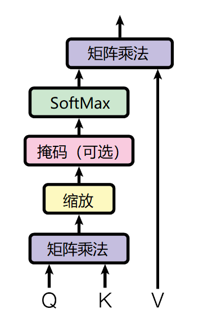
\includegraphics[scale = 0.8]{figures/DotAtt}
	\caption{缩放点积注意力}
	\label{fig:DotAtt}
\end{figure}

具体落实在实践中,对于一组亟待查询的注意力函数,应当将这些查询同时计算,封装到一个矩阵 $Q$ 中。键和值也封装到矩阵 $K$ 和 $V$ 中。这样在具体计算中,就可以使用矩阵乘法的方法来予以优化。这样的话,可以把注意力函数中输出的矩阵计算为:
\begin{equation}
\text{Attention}(Q,K,V) = \text{softmax}(\frac{QK^T}{\sqrt{d_k}})V
\label{eq3.1}
\end{equation}

在 Transformer 之前的研究中,加法注意和点积的乘法注意是在此之前最常用的两个注意力函数。点积注意力与 Transformer 的缩放点积注意力算法相比,除了 $\frac{1}{\sqrt{d_k}}$ 的比例因子之外,都差不多,没有什么不同。加法注意的方法在计算的时候使用具有单个隐藏层的前馈网络。即使加法注意和点积注意这两个注意力方法在理论上的复杂性相似,但是点积注意力由于使用可以并行化且优化非常棒的矩阵乘法来实现,所以在实践中代码跑的更快且代码更节省空间一些。

在查询和键的维度数 $d_k$ 较小的时候,这两种机制的性能相似。但是在 Transformer 原论文中有提及,查询和键的维度数 $d_k$ 较大时,矩阵相乘后的造成的矩阵中的元素的值会变大,进而使得经过 softmax 函数后的矩阵中的每个元素的梯度反而变得更小,更难以训练且难以出结果。为了抵消这种影响,我们将点积乘上 $\frac{1}{\sqrt{d_k}}$,以缩小其中元素的值。

(2) 多头注意力

其实,如果将键、值和查询都使用 $d_{\text{model}}$ 维度的话,相比于将查询、键和值直接投影到 $d_k$、$d_k$ 和 $d_v$ 维度上做不同的学习线性投影实际上是对这个模型反而是会变得更劣。在此之后,在每个查询、键和值的投影向量上,代码并行地执行注意力函数,并产生 $d_v$ 维输出值。上一步输出出来的 $d_v$ 维输出值被连接起来并再次投影,再输出出去,具体过程如图 \ref{fig:MultiheadAtt} 所示。

\begin{figure}[htbp]
	\centering
	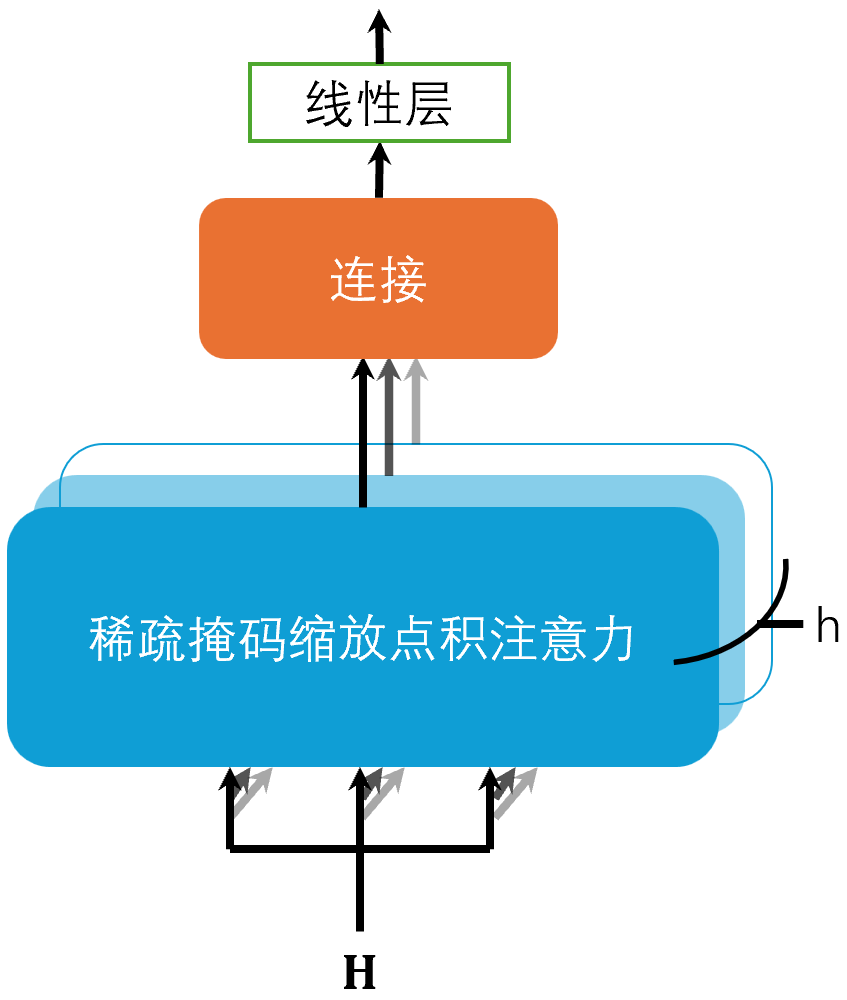
\includegraphics[scale = 0.8]{figures/MultiheadAtt}
	\caption{多头注意力}
	\label{fig:MultiheadAtt}
\end{figure}

多头注意力的优点就是可以让注意力模型可以同时关注在不同位置上的信息。而如果只有单个注意力头的话,平均化会抑制这一点。
\begin{equation}
\text{MultiHead}(Q, K, V) = \text{Concat}(\text{head}_1, ..., \text{head}_h)W^O
\label{eq3.2}
\end{equation}
\begin{equation}
\text{head}_i = \text{Attention}(QW_i^Q, KW_i^K, VW_i^V)
\label{eq3.3}
\end{equation}
其中投影是参数矩阵 $W_i^Q \in \mathbb{R}^{d_{\text{model}}}, W_i^K \in \mathbb{R}^{d_{\text{model}} \times d_k}, W_i^V \in \mathbb{R}^{d_{\text{model}} \times d_v}, W^O \in \mathbb{R}^{hd_v \times d_{\text{model}}}$

在 Transformer 中,使用了 $h = 8$ 个并行注意力层或头。对于其中的每一个,使用 $d_k = d_v = d_{\text{model}} / h = 64$。由于每个头的维度减少,总计算成本类似于具有全维度的单头注意力。

\subsection{位置前馈网络}
除了注意力子层之外,编码器和解码器中的每一层都包含一个完全连接的前馈网络,该网络分别且相同地应用于每个位置。这包括两个线性变换,中间有一个线性整流函数(ReLU)激活。
\begin{equation}
\text{FFN}(x) = \max(0, xW_1 + b_1)W_2 + b_2
\label{eq3.4}
\end{equation}

虽然线性变换在不同位置上是相同的,但它们在层与层之间使用不同的参数。另一种描述方式是内核大小为 $1$ 的两个卷积。输入和输出的维数为 $d_{\text{model}} = 512$,内层的维数为 $d_{ff} = 2048$。

\subsection{嵌入层和 softmax 函数}

与其他序列转导模型类似,Transformer 使用学习嵌入将输入序列中的词汇和输出序列中的词汇转换为维度 $d_{\text{model}}$ 的向量。除此之外,还使用了通常的学习线性变换和 softmax 函数将解码器输出转换为预测的下一个词汇的概率。在我们的模型中,我们在两个嵌入层和 pre-softmax 线性变换之间共享相同的权重矩阵。在嵌入层中,我们将这些权重乘以 $\sqrt{d_{\text{model}}}$。也有使用 log-softmax 函数替代 softmax 函数的情况。

\subsection{位置编码}

由于 Transformer 模型不包含递归和卷积,为了让模型利用序列的顺序,必须注入一些关于标记在序列中的相对或绝对位置的信息。为此,我们在编码器和解码器堆栈底部的输入嵌入中添加“位置编码”。位置编码与嵌入具有相同的维度 $d_{\text{model}}$,因此可以将两者相加。位置编码有很多选择,由模型学习出来的或是公式计算固定出来的。

在 Transformer 中,使用不同频率的正弦和余弦函数:
\begin{equation}
\begin{aligned}
\text{PE}(pos,2i) &= \sin \left ( \frac{pos}{10000^{2i/d_{\text{model}}}} \right ) \\
\text{PE}(pos,2i+1) &= \cos \left ( \frac{pos}{10000^{2i/d_{\text{model}}}} \right )
\end{aligned}
\label{eq3.5}
\end{equation}
其中 $pos$ 是位置,$i$ 是维度。也就是说,位置编码的每个维度对应一个正弦曲线。波长形成从 $2\pi$ 到 $10000 \cdot 2\pi$ 的几何级数。我们选择这个函数是因为我们假设它可以让模型轻松学习通过相对位置来参与运算,因为对于任何固定的偏移量 $k$,$\text{PE}_{pos+k}$ 可以表示为 $\text{PE}_{pos}$ 的线性函数。

使用公式固定计算出来的正弦版本好处有,它可以让模型推断出比训练期间遇到的序列长度更长的序列长度。

\subsection{最后的线性层}
数据通过 log-softmax 函数之后,将通过一层线性层将这个维度为 $d_{\text{model}}$ 的向量转化为维度为词汇个数的向量,该向量表示下一个预测的词汇是什么。

\section{预训练语言模型技术}

近年来,自然语言处理((Natural Language Processing,NLP)的发展取得了巨大进步,其中预训练语言模型(PLMs,Pre-trained Language Models)的研究为自然语言处理的进展提供了关键支持。其核心概念是首先在大型数据集上对深度神经网络进行预先训练,以获取模型参数,然后利用这些经过训练的模型来执行各种具体的下游任务,从而避免从头开始训练模型并减少对标注数据的需求量。与预训练语言模型思想相关的早期工作可以追溯到 NNLM \cite{NNLM} 和 word2Vector \cite{mikolov2013efficientestimationwordrepresentations},2017 年 Vaswani 等人 \cite{transformer} 提出了 Transformer,基于 Transformer 的预训练语言模型大大提高了各种 NLP 任务的性能,由此 Transformer 成为各种预训练语言模型的主干。基于 Transformer 的编码端(Encoder),Radford 等人 \cite{gpt} 提出了 GPT 模型,GPT 真正意义上实现了预训练-微调的框架,不再需要将模型中的词嵌入取出来,而是直接把预训练好的模型在下游任务上微调,对于不同任务采用不同的输入或对输出层改造,让下游任务更贴近上游预训练模型,目前 GPT 模型的应用取得了巨大成功,各种 GPT 大模型层出不穷,给 NLP 等领域注入了新的活力。Devlin 等人 \cite{devlin_bert_2019} 基于 Transformer 的 Encoder 编码端提出 BERT 模型,也是目前在 NLP 中应用最广泛的预训练模型之一,BERT 采用了一种 Mask Language Model(MLM)的方法,通过随机 mask 掉输入文本中的某些词元,然后利用上下文信息进行预测,实现对数据语义关系的提取。继 GPT 和 BERT 之后,研究人员又提出了 XLNet \cite{XLNet}、RoBERTa \cite{liu_roberta_2019}、DeBERTa \cite{he_deberta_2021} 、ERNIE \cite{sun2019ernieenhancedrepresentationknowledge}、T5 \cite{T5} 和 BART \cite{lewis-etal-2020-bart} 等预训练语言模型。本节将对本文所使用模型 RoBERTa 和 DeBERTa 的基础模型 BERT 预训练语言模型进行介绍。

% 写写 BERT 吧
BERT(Bidirectional Encoder Representation from Transformers)\cite{devlin_bert_2019} 是2018年10月由Google AI研究院提出的一种预训练模型,该模型在机器阅读理解顶级水平测试SQuAD1.1 \cite{rajpurkar2016squad100000questionsmachine} 中表现出惊人的成绩: 全部两个衡量指标上全面超越人类,并且在11种不同NLP测试中创出SOTA表现,包括将GLUE基准 \cite{wang2019gluemultitaskbenchmarkanalysis} 推高至80.4\% (绝对改进7.6\%),MultiNLI 数据集 \cite{williams2018broadcoveragechallengecorpussentencemultinli} 准确度达到86.7\% (绝对改进5.6\%),成为NLP发展史上的里程碑式的模型成就。BERT 在 Transformer 的基础上引入了预训练和微调的策略,使得模型在预训练阶段学习通用的语言表示,而在特定任务中进行微调,极大地提升了模型的适应性和性能。因此,尽管 BERT 不是第一个预训练模型,但它在预训练模型的发展历程中具有里程碑式的意义。

\subsection{BERT 结构}

BERT 在 Transformer 基础上做的改进不多,采用了 Transformer 编码器的结构作为基础结构。总体结构图如 \ref{fig:BERT} 所示,多个Transformer 编码器层一层一层地堆叠起来,就是 BERT 的总体结构了,在原始论文中,作者分别用12层和24层Transformer 编码器组装了两套 BERT 模型,110M和340M分别为两套模型的总参数。

\begin{figure}[htbp]
	\centering
	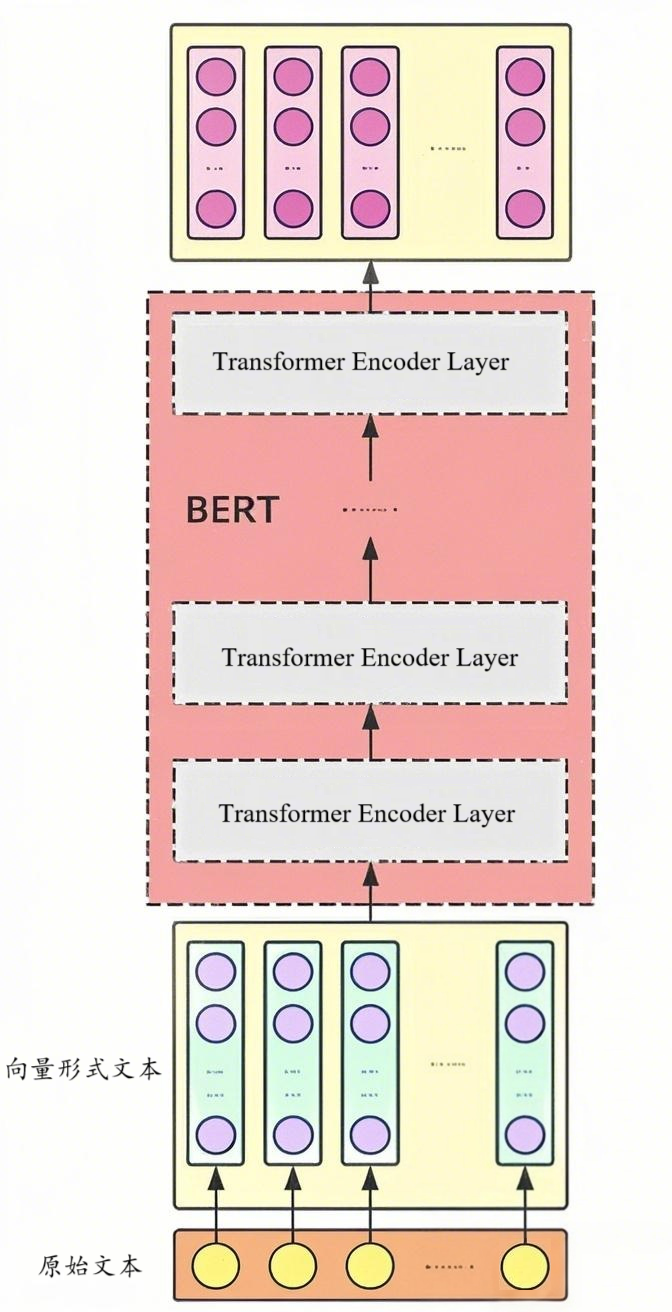
\includegraphics[scale = 0.7]{figures/bert.png}
	\caption{BERT 架构图}
	\label{fig:BERT}
\end{figure}

\subsection{嵌入}

对于 BERT 而言,一个巨大的改进就是其嵌入(Embedding)上的改进。为了使 BERT 能够处理多种下游任务,BERT 的输入表示能够在一个词元序列中清晰地表示单个句子和一对句子(例如,〈问题,答案〉)。在整个工作中,“句子”可以是一个任意跨度的连续文本,而不是一个实际的在自然语言意义下的句子。“序列(sequence)”是指输入 BERT 的词元序列,它可能是单个句子,也可能是多个句子打包在一起。

在 BERT 中使用带有 30,000 个词元词汇表的 WordPiece 嵌入。每个序列的第一个标记始终是一个特殊的分类标记([CLS])。与此标记对应的最终隐藏状态用作分类任务的聚合序列表示。最后一层该位对应向量可以作为整句话的语义表示,从而用于下游的分类任务等。因为与文本中已有的其它词相比,这个无明显语义信息的符号会更“公平”地融合文本中各个词的语义信息,从而更好的表示整句话的语义。 具体来说,self-attention是用文本中的其它词来增强目标词的语义表示,但是目标词本身的语义还是会占主要部分的,因此,经过BERT的12层(BERT-base为例),每次词的embedding融合了所有词的信息,可以去更好的表示自己的语义。而[CLS]位本身没有语义,经过12层,句子级别的向量,相比其他正常词,可以更好的表征句子语义。在 BERT 执行过程中,句子对被打包到一个单一的序列中。在此情况下,通过两种方式对句子进行区分。首先,用一个特殊的标记([SEP])将它们分开。其次,BERT 将学习到的嵌入添加到每个词元中,指示它是属于句子A还是句子B。

\begin{figure}[htbp]
	\centering
	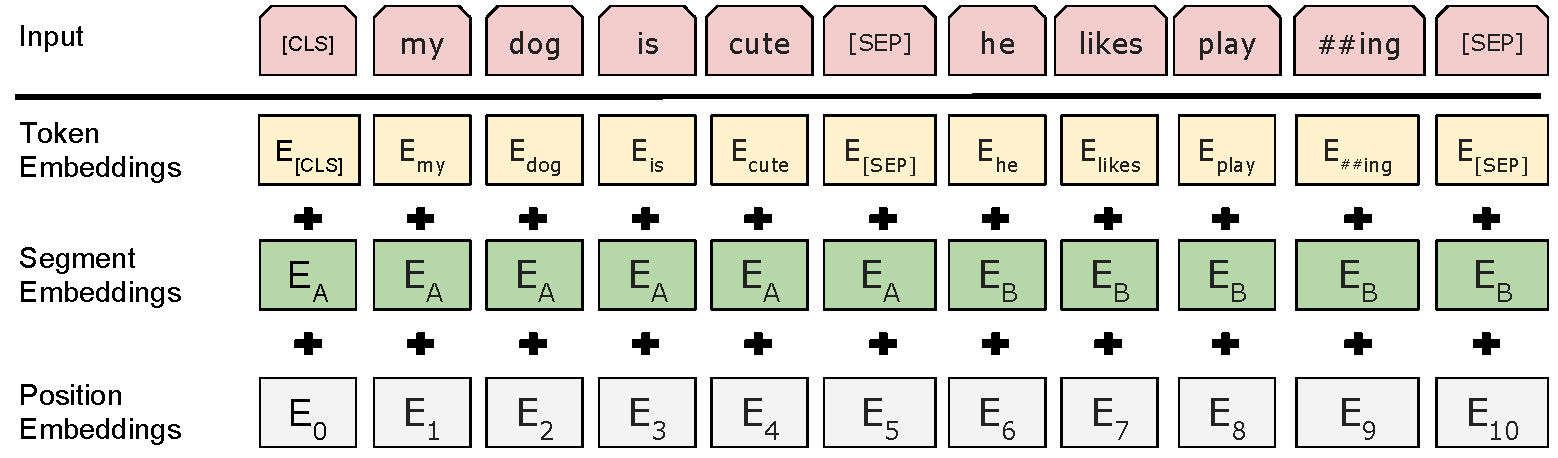
\includegraphics[width=\linewidth]{figures/bert_Input_Emebeddings.pdf}
	\caption{BERT 嵌入(Embedding)示意图}
	\label{fig:BERT-embedding}
\end{figure}

对于给定的词元,其输入表示(input representation)是通过对相应的词元(token)、段(segment)和位置(position)嵌入进行求和来构造的。这个结构的可视化如图 \ref{fig:BERT-embedding} 中所示。

\subsection{预训练与微调}

BERT 这项工作最大的贡献是将二阶段训练过程发扬光大,其训练过程分为预训练过程(pretraining)和微调过程(finetuning),训练过程示意图如图 \ref{fig:BERT-OverAll} 所示。预训练阶段旨在通过大规模的无标注文本数据来学习语言的深层次表示,BERT采用了带掩码的语言模型(Masked Language Model,MLM)和下一句预测(Next Sentence Prediction,NSP)两种任务,使模型能够理解上下文的双向信息。在微调阶段,BERT 可以针对特定任务进行调整,只需在少量标注数据上进行训练,从而能够高效地适应多种自然语言处理任务,如文本分类、问答系统和命名实体识别等。

\begin{figure}[htbp]
	\centering
	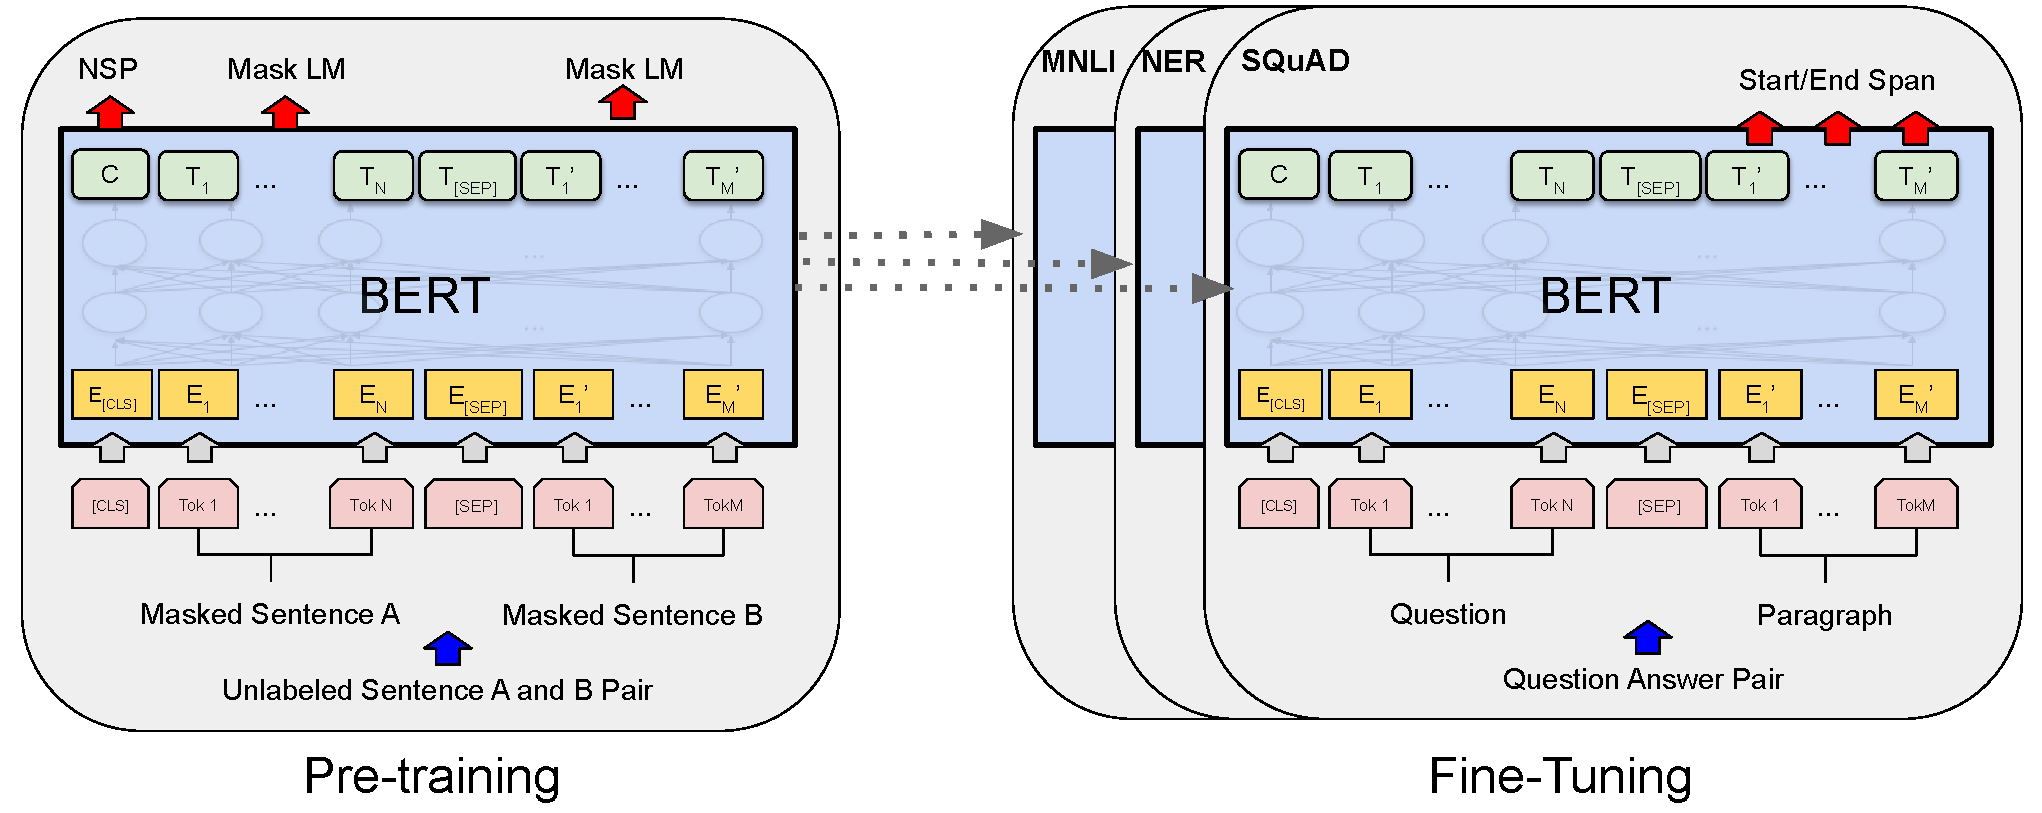
\includegraphics[width=\linewidth]{figures/BERT_Overall.pdf}
	\caption{BERT 训练过程示意图}
	\label{fig:BERT-OverAll}
\end{figure}

这种预训练-微调的二阶段训练范式显著提升了模型在各种NLP任务上的性能,标志着自然语言处理领域的一次重大变革。BERT的成功也激励了后续大量基于Transformer架构的预训练模型的研发,例如本文要使用的 RoBERTa 和 DeBERTa,以及其他在 BERT 模型上做出改进的模型,这些模型在不同的任务中展示了更高的效率和准确性。通过这些创新,BERT不仅推动了学术界对预训练模型的研究,也促进了工业界在实际应用中的广泛采用。

\section{AI 生成文本探测技术}
\label{sec:llmdetect}

大型语言模型(LLMs)的快速发展推动了对检测AI生成文本方法的深入研究。在ChatGPT问世之前,GLTR \cite{gehrmann_gltr_2019} 作为一种检测工具,通过一系列统计方法识别由不同采样方案生成的文本伪影。GLTR 有效地将人类对生成文本的检测率从54\%提升至72\%,突显了其在帮助非专家区分人类与机器生成内容方面的实用性。

另一个重要贡献是人类ChatGPT比较语料库 \cite{guo_how_2023}(HC3),该语料库是在ChatGPT出现后开发的。HC3数据集包含来自人类专家和ChatGPT的数万个响应,涵盖金融、医学和法律等多个领域。这一数据集使得对ChatGPT的响应与人类输出进行全面评估成为可能,揭示了LLMs的能力与局限性。此外,HC3还促进了检测系统的发展,旨在识别文本是由ChatGPT还是人类生成的。

LLM-Detector \cite{wang_llm-detector_2024} 则解决了现有人工智能生成文本检测模型面临的挑战,这些模型通常因领域内过拟合而在领域外表现不佳。该研究通过收集人类专家和各种大语言模型的回复,依托于大型语言模型提出了一种新颖的检测方法,利用指令调优来增强文档级和句子级的检测能力。实验结果表明,该方法在性能上显著优于基线方法,展现了强大的泛化能力。

SeqXGPT \cite{wang_seqxgpt_2023} 通过合成一个包含大语言模型生成句子和人类写作内容的数据集,引入了句子级检测挑战。该方法利用来自白盒LLMs的对数概率列表,结合卷积和自注意力网络来提高检测准确性。结果显示,SeqXGPT在句子和文档级检测任务中均优于现有方法,进一步强调了有效检测机制的必要性。

针对人工智能生成文本的来源追踪问题 \cite{li_origin_2023},有研究提出了一种新颖的算法,用于检测和追踪人工智能生成的内容。该方法利用对比特征来区分由不同模型生成的文本,能够在白盒和黑盒环境中有效运行。研究结果强调了人工智能部署的伦理影响以及追踪生成文本来源机制的必要性,为有关人工智能系统问责制的持续讨论提供了重要依据。

然而,现有的方法 \cite{gehrmann_gltr_2019, guo_how_2023, wang_llm-detector_2024, wang_seqxgpt_2023} 未能满足我们对文本来源于特定大型语言模型的检测需求。大多数研究在分类任务上表现较为粗糙,仅能识别文本是由人类还是机器生成,无法进一步确定文本的具体来源。尽管少部分研究 \cite{li_origin_2023} 实现了识别文本来源于特定大型语言模型的目标,但其实现方式依赖于白盒测试,必须获取与待检测模型一致或相似的模型生成的特征向量才能进行判断。在当前大多数大型语言模型均为闭源的环境下,这种方法几乎缺乏扩展性和可操作性。

\section{本章小结}
\label{sec:rw-conclusion}

本章回顾了当前自然语言处理领域的相关工作,重点聚焦于文本生成技术和预训练语言模型的进展。首先,我们深入分析了Transformer架构的优势,强调了其在大语言模型中的广泛应用。自2017年提出以来,Transformer因其卓越的并行处理能力和长距离依赖建模能力,迅速成为自然语言处理研究的核心。通过自注意力机制,Transformer能够有效捕捉输入序列中各个部分之间的关系,从而显著提高了模型在处理大规模文本数据时的训练效率和表达能力。

随后,我们详细讨论了BERT模型的结构及其在预训练和微调过程中的创新。BERT不仅在机器阅读理解等多个任务中取得了显著的性能提升,还引入了预训练-微调的二阶段训练范式,使得模型能够在预训练阶段学习通用的语言表示,而在特定任务中进行微调。这一策略极大地提升了模型的适应性和性能,标志着自然语言处理领域的一次重大变革。在预训练语言模型的讨论中,我们提及了如GPT、RoBERTa和DeBERTa等模型的相继出现,这些模型在BERT的基础上进行了不同程度的改进,进一步推动了预训练模型的研究和应用。

最后,本章探讨了AI生成文本的检测技术,介绍了多种现有方法及其在实际应用中的效果与局限性。尽管GLTR、HC3、LLM-Detector、SeqXGPT等工具在识别生成文本方面取得了一定的成效,但仍面临特定大型语言模型检测的挑战。尤其是在当前许多大型语言模型为闭源的环境下,现有方法在文本来源追踪和特定模型检测方面的适用性显得尤为重要。

综上所述,本章的讨论为理解当前技术状态及未来研究方向提供了重要视角,为本论文的研究奠定了坚实的基础。通过对Transformer架构、BERT模型及AI文本检测技术的全面回顾,我们为后续的研究和实验提供了必要的理论支持和实践指导。